\documentclass[11pt,a4paper]{article}

\usepackage[margin=24mm]{geometry}
\usepackage{graphicx}
\usepackage{amsmath}
\usepackage{booktabs}
\usepackage{longtable}
\usepackage{tabularx}
\usepackage{array}
\usepackage{float}
\usepackage{caption}
\usepackage{subcaption}
\usepackage{placeins}
\usepackage{xcolor}
\usepackage{enumitem}
\usepackage[hidelinks]{hyperref}

\graphicspath{{fig/}}
\setlength{\parindent}{0pt}
\setlength{\parskip}{6pt}
\setlist[itemize]{leftmargin=*, topsep=2pt}
\setlist[enumerate]{leftmargin=*, topsep=2pt}

\newcommand{\mm}{\,\mathrm{mm}}
\newcommand{\Hz}{\,\mathrm{Hz}}
\newcommand{\pct}{\,\%}
\newcommand{\case}[1]{\texttt{#1}}
\newcommand{\tight}{\setlength{\tabcolsep}{4pt}\renewcommand{\arraystretch}{1.12}}

\title{\textbf{AutoPos UWB Field Evaluation Report}\\
\large OptiTrack-Isolated Static, Dynamic, Delay, Filtering, and Robustness Analysis}
\author{FULL Erlangen 2026-05-28 analysis package}
\date{Generated from the corrected FULL 4-way comparison and reviewer-audit outputs, 2026-06-04}

\begin{document}
\maketitle

\begin{abstract}
This report summarizes the corrected FULL AutoPos/Vicon analysis for the Erlangen
2026-05-28 dataset.  The evaluation separates anchor-layout accuracy, residual
delay/layout coupling, static tag positioning, dynamic ROTO trajectory tracking,
post-solve filtering, pseudo-IMU oracle fusion, and robustness diagnostics.  The
main deployment headline is the production mean-aggregated static point after the
real production export path was switched to the T4 tag solver:
\textbf{72.7 mm median, 171.5 mm P95, and 109.8 mm RMSE} for original FULL
\case{v4-io/T4}.  The older \textbf{69.7/173.9 mm} result is retained only as a
median-estimator ablation, not as the deployed production statistic.  Dynamic
ROTO absolute trajectory error remains about \textbf{105.8 mm median and
231.8 mm track-level P95} on the same \case{v4-io/T4} solver line, showing that
dynamic error does not collapse simply by improving anchor geometry.
The FULL-US rerun represents the BioSpur AutoPos deployment system with UWB plus
the US30/F-G-H height gauge.  It does not materially change the legacy 3D
anchor-locked accuracy numbers; instead, it fixes the vertical gauge so that the
coordinate frame is physically interpretable.  Under the new height-preserving
evaluation, FULL-US \case{v4-io} gives \textbf{72.5 mm median, 284.8 mm P95,
and 139.1 mm RMSE} for static tag points against OptiTrack.
\end{abstract}

\section{One-Page Result Summary}

\begin{table}[H]
\centering
\tight
\caption{Primary results.  Static production uses mean aggregation per static position.
ROTO values are track-median summaries over 34 tag tracks from 17 rotating captures.}
\begin{tabularx}{\textwidth}{lXrrr}
\toprule
Domain & Case & Median/P50 & P95 & RMSE or key diagnostic \\
\midrule
Static deployed headline & FULL production mean-aggregated \case{v4-io/T4} & 72.7 & 171.5 & 109.8 RMSE \\
Static deployment gauge & FULL-US UWB+US30 height-preserving \case{v4-io} & 72.5 & 284.8 & 139.1 RMSE \\
Anchor deployment gauge & FULL-US UWB+US30 height-preserving \case{v4-io} & 98.4 & 162.1 & 109.7 RMSE \\
Static legacy production & FULL production mean-aggregated \case{v4-io/T1} & 74.0 & 282.1 & 139.6 RMSE \\
Static estimator ablation & FULL median-estimator \case{v4-io/T4} & 69.7 & 173.9 & 108.9 RMSE \\
Known-anchor control & Vicon anchors + re-estimated delay, T4 & 64.1 & 128.4 & 77.7 RMSE \\
One-baseline control & E-H one-baseline + re-estimated delay, T4 & 58.1 & 130.2 & 78.4 RMSE \\
ROTO baseline & FULL original \case{v4-io/T4} & 105.8 & 231.8 & 141.3 sample RMSE \\
ROTO known-anchor control & Vicon anchors + re-estimated delay, T4 & 105.6 & 200.4 & 125.4 sample RMSE \\
ROTO fixed-lag filter & FULL original \case{T4+F4} & 86.3 & 158.2 & diagnostic latency smoother \\
ROTO pseudo-IMU oracle & FULL original \case{T4+PI1} & 66.1 & 97.5 & OptiTrack-derived motion prior \\
\bottomrule
\end{tabularx}
\end{table}

The most important interpretation is that the system has two different regimes:
static tag localization benefits strongly from correct layout/delay handling and
from static dwell aggregation, while ROTO remains a roughly 10 cm absolute dynamic
trajectory problem even under known-anchor controls.  The dynamic residual is not
mainly a constant time-offset problem, not mainly the 0.8 ms protocol broadcast
window, and not mainly a global anchor-layout scale problem.

\section{FULL-US: UWB Plus US30 Height Gauge}

The original FULL analysis and the FULL-US rerun answer slightly different
questions.  Original FULL \case{v4-io} is the UWB AutoPos self-calibration with
the historical soft two-layer vertical prior.  FULL-US \case{v4-io} is the same
AutoPos pipeline after applying the US30/F-G-H ultrasound height gauge to fix
the vertical coordinate gauge.  OptiTrack remains the external ground truth.

\begin{table}[H]
\centering
\tight
\caption{FULL, FULL-US, and OptiTrack compared.  Values are 3D errors in mm
against OptiTrack where applicable.}
\begin{tabularx}{\textwidth}{lXrrr}
\toprule
System & Coordinate meaning & Static tag P50/P95 & Anchor P50/RMSE & ROTO P50/P95 \\
\midrule
FULL \case{v4-io} & UWB AutoPos with soft two-layer Z prior; gauge is not a directly deployed height frame & 74.0/282.1 legacy production & 92.8/105.4 & 105.8/231.8 \\
FULL-US \case{v4-io} & UWB AutoPos plus US30/F-G-H height gauge; vertical gauge is deployment-interpretable & 72.5/284.8 height-preserving & 98.4/109.7 height-preserving & 105.8/231.8 \\
OptiTrack & Optical ground truth reference & reference & 0.28 mm coordinate-SD median & reference \\
\bottomrule
\end{tabularx}
\end{table}

The important result is that FULL-US is not a large accuracy-improvement module
under the old metric.  In the no-US versus US comparison, 8 of 10 legacy
anchor-locked rows are numerically unchanged, and the remaining two change by
less than 0.12 mm in P95.  This is expected: a full 3D anchor/capture alignment
can absorb a gauge-only coordinate-frame change.

Therefore the US30 contribution should be worded as follows.  It fixes the
BioSpur AutoPos coordinate gauge, especially the vertical axis, so that the
output coordinate system is physically interpretable in deployment.  It does not
by itself make UWB ranging substantially more accurate.  The correct deployment
diagnostic is the height-preserving check: only a horizontal 2D rigid transform
plus a vertical shift is allowed, so arbitrary 3D pitch/roll cannot erase the
US height gauge.  Under this check, FULL-US \case{v4-io} has static tag error
72.5/284.8 mm with 139.1 mm RMSE, and anchor layout error 98.4/162.1 mm with
109.7 mm RMSE.

\section{Dataset, Reference Frames, and Evaluation Protocol}

The dataset is the corrected FULL OptiTrack export from Erlangen on 2026-05-28.
The main infrastructure configuration is AutoPos \case{v4-io}, evaluated against
OptiTrack/Vicon anchor and tag truth.  The analysis compares four major paths:
\begin{itemize}
    \item original FULL self-calibrated AutoPos layout with solver residual corrections;
    \item known Vicon/OptiTrack anchor coordinates with residual delay re-estimated on that frame;
    \item full Sim(3) scale-to-Vicon layout with residual delay re-estimated;
    \item one-baseline E-H scale correction with residual delay re-estimated.
\end{itemize}

Static results summarize 24 fixed tag positions.  ROTO results summarize 34
tag tracks from 17 rotating captures.  Static production results use the actual
production export path: every static frame is solved, then the final static point
is the mean of the solved coordinates in \case{position\_summary}.  The production
path was switched from the legacy T1 analytic solver to the T4 C-solver, while
mean aggregation was intentionally kept unchanged.  This real production run
reproduced the probe result within numerical noise:
\[
72.691/171.493/109.843\mm \quad \text{real run}
\]
versus
\[
72.689/171.497/109.845\mm \quad \text{probe}.
\]

\section{Metric Definitions}

\begin{itemize}
    \item \textbf{Static median/P95/RMSE:} 3D error between the estimated static tag
    point and the corrected OptiTrack tag truth.
    \item \textbf{ROTO ATE:} absolute trajectory error between solved UWB antenna
    samples and interpolated OptiTrack antenna markers.
    \item \textbf{ROTO track-median:} the median of per-track summary values, used
    to avoid over-weighting longer tracks.
    \item \textbf{RPE:} frame-to-frame relative position error, used as a local
    motion consistency metric.
    \item \textbf{SE(3) layout error:} rigid/reflection-normalized anchor error
    against OptiTrack layout.  It preserves global scale bias.
    \item \textbf{Sim(3) layout error:} similarity residual after allowing one global
    scale factor.  It measures non-uniform shape distortion after removing global scale.
    \item \textbf{Delay correction:} all \case{d\_anchor\_mm} and tag-delay terms
    in this report are layout-level residual software corrections fitted on top of
    the firmware antenna-delay setting 16436 DTU.  They are not quoted as physical
    antenna delays.
\end{itemize}

\section{Anchor Self-Positioning Accuracy}

\begin{figure}[H]
\centering
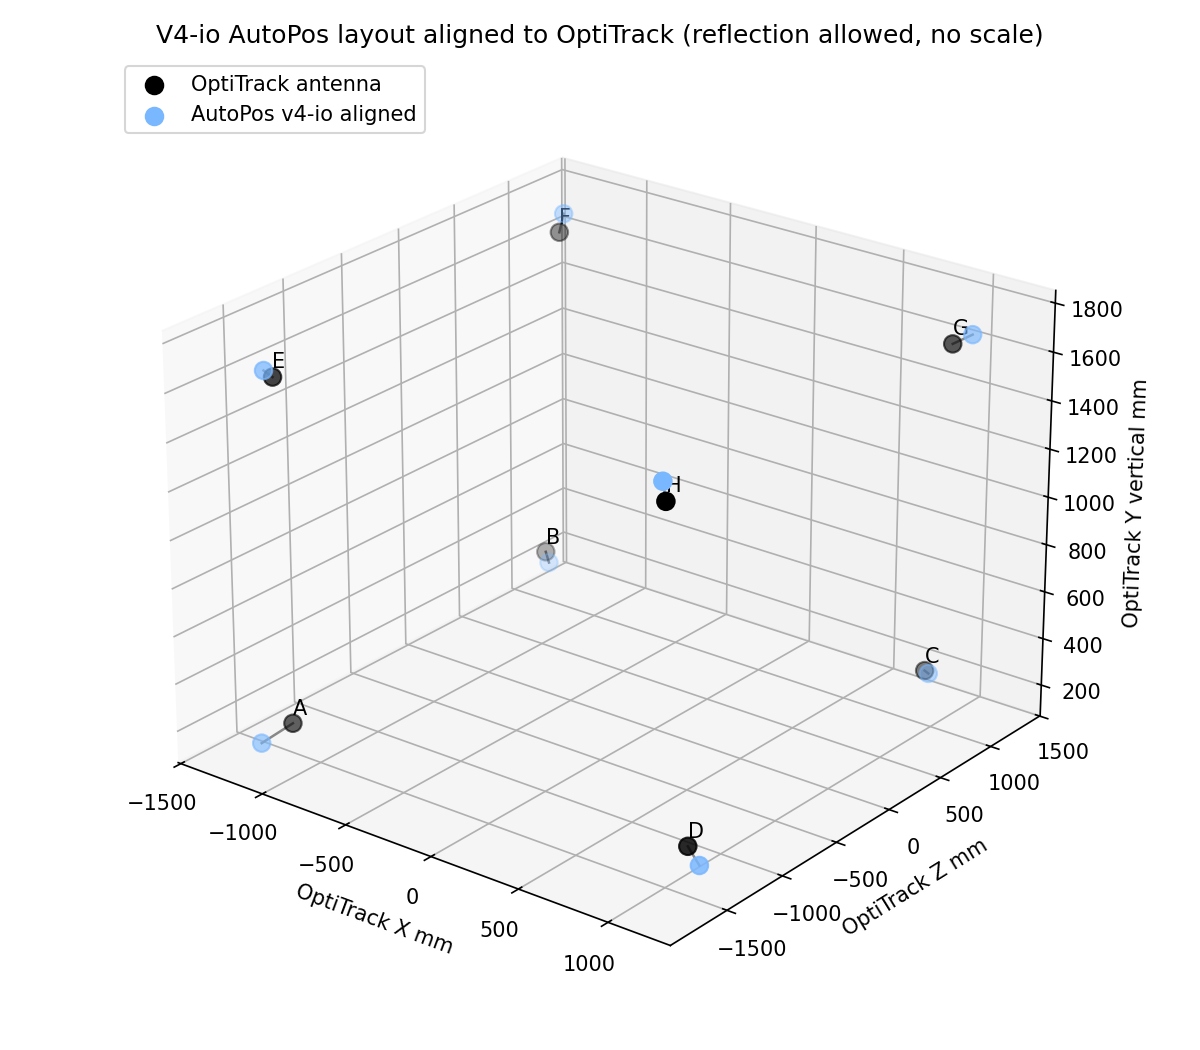
\includegraphics[width=0.88\textwidth]{layout_opti_vs_autopos_3d.png}
\caption{OptiTrack anchor layout versus AutoPos layout.  The key point is not only
the 3D anchor coordinate error but also the global scale shrinkage visible after
alignment.}
\end{figure}

\begin{table}[H]
\centering
\tight
\caption{Anchor layout absolute accuracy.  SE(3) preserves scale bias; Sim(3)
removes a single global scale degree of freedom.}
\begin{tabular}{lrrrrr}
\toprule
Method & SE(3) RMSE & Median & P95 & Scale bias & Sim(3) RMSE \\
\midrule
AutoPos v1-old & 101.3 & 84.6 & 154.1 & -4.50\% & 50.1 \\
AutoPos v4-io & 105.4 & 92.8 & 156.9 & -4.17\% & 67.1 \\
AutoPos v2 & 136.5 & 127.8 & 184.0 & -6.15\% & 60.3 \\
AutoPos v3-lite & 136.6 & 127.9 & 184.2 & -6.15\% & 60.9 \\
AutoPos v3-full & 143.4 & 118.9 & 211.7 & -3.61\% & 125.3 \\
\bottomrule
\end{tabular}
\end{table}

The production layout \case{v4-io} has a frame-normalized rigid SE(3) RMSE of
105.4 mm and a Sim(3) residual of 67.1 mm.  The Sim(3) scale is 0.958267, meaning
the AutoPos layout is globally about 4.17\% smaller than the OptiTrack layout.
Therefore the gap between rigid and similarity RMS is not a computation bug; it
is the scale degree of freedom doing real work.  In paper text, the similarity
number should be marked as diagnostic rather than as deployed field accuracy.

\section{Delay-Layout Coupling}

\begin{figure}[H]
\centering
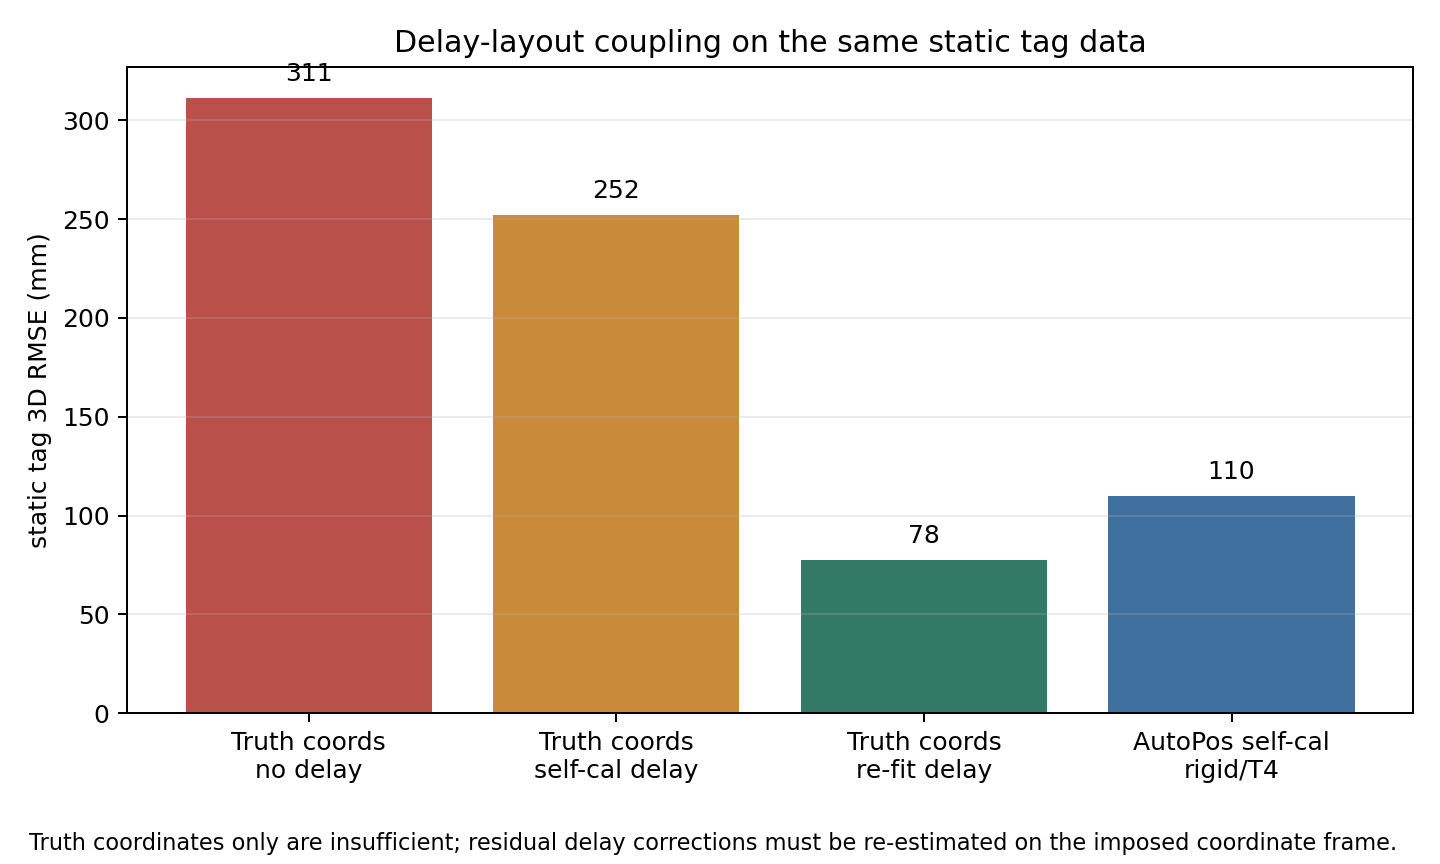
\includegraphics[width=0.78\textwidth]{delay_layout_coupling.png}
\caption{Delay-layout coupling triangle.  Imposing optical anchor coordinates is
not enough; residual delay must be re-estimated on the imposed coordinate frame.}
\end{figure}

\begin{table}[H]
\centering
\tight
\caption{Same static tag data under different layout and delay treatments.}
\begin{tabularx}{\textwidth}{lXrr}
\toprule
Case & Interpretation & RMSE & P95 \\
\midrule
Vicon truth, no delay correction & Optical geometry alone is insufficient & 311.3 & 453.4 \\
Vicon truth, transplanted self-cal delay & AutoPos residual corrections are not portable & 252.2 & 394.6 \\
Vicon truth, re-estimated delay & Known-anchor + re-estimated-delay control & 77.7 & 128.4 \\
AutoPos v4-io, co-fitted delay & Self-cal geometry and delay are jointly conditioned & 108.9 & 174.1 \\
\bottomrule
\end{tabularx}
\end{table}

This is the central contribution of the OptiTrack-isolated analysis.  Known anchor
coordinates by themselves do not solve the tag problem; the endpoint residual
delay model must be re-estimated in the same layout frame.  The mechanism is also
visible at the per-anchor level: WHY \#9 regresses self-minus-Vicon
\case{anchor\_main\_rel\_A} on \case{v4-io} radial layout error and obtains
\(R^2=0.998\) with slope \(-0.982\mm/\mm\).  In other words, the self-cal residual
delay term absorbs radial coordinate and scale error almost one-to-one.  This is
not a solver sign bug; it is gauge absorption.

\section{Static Tag Positioning}

\begin{figure}[H]
\centering
\begin{subfigure}{0.49\textwidth}
\centering
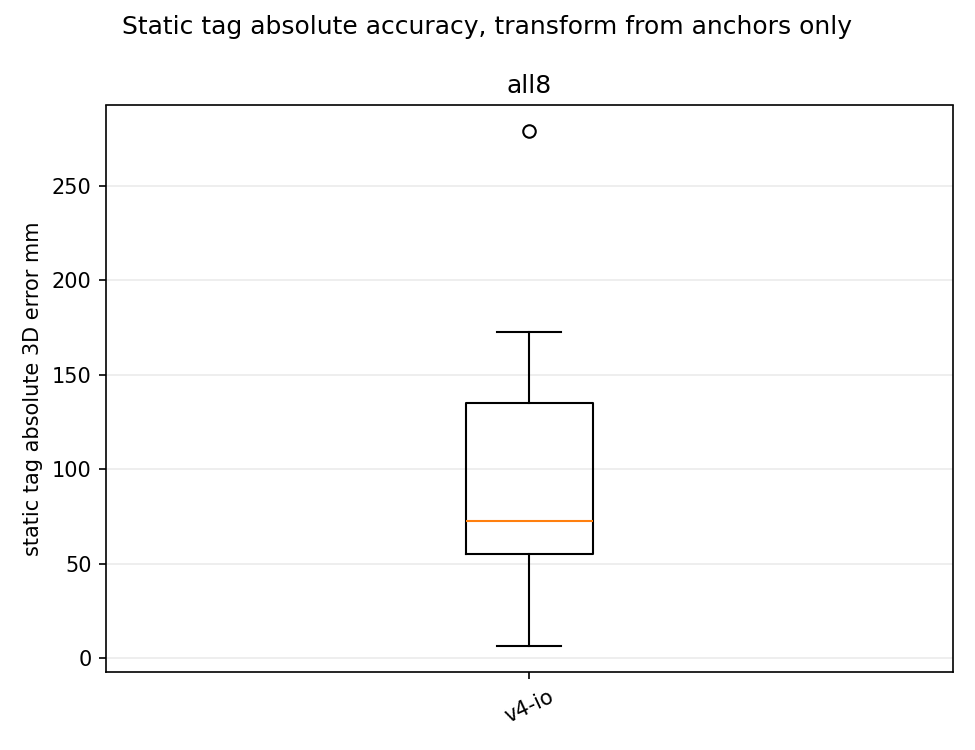
\includegraphics[width=\linewidth]{production_T4_tag_error_by_position.png}
\caption{Production T4 mean-aggregated static error by position.}
\end{subfigure}
\hfill
\begin{subfigure}{0.49\textwidth}
\centering
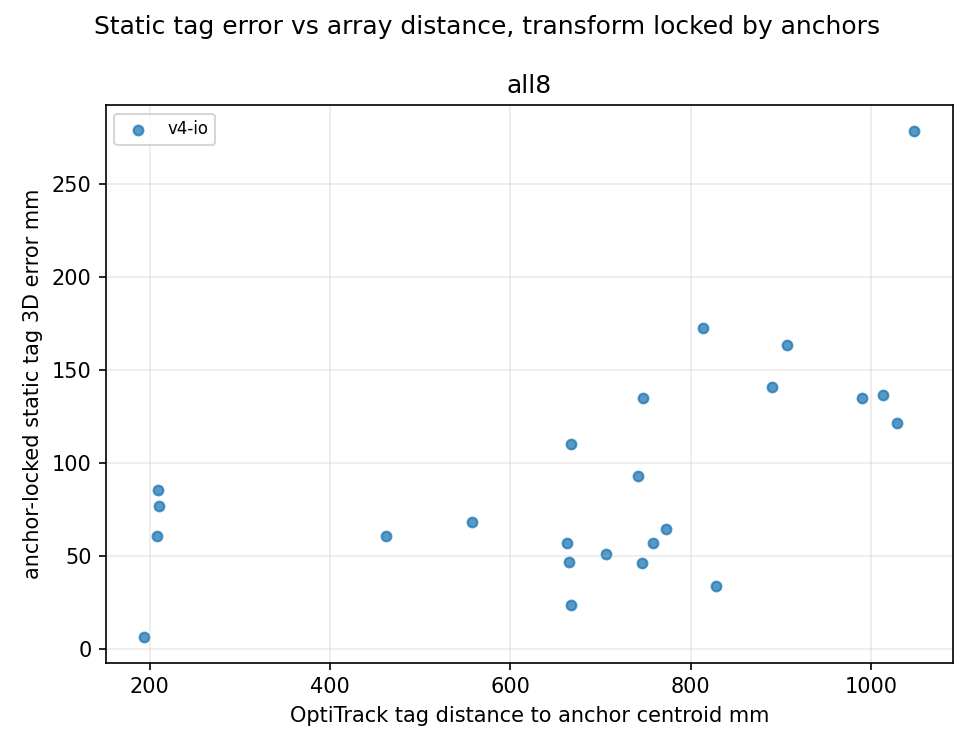
\includegraphics[width=\linewidth]{production_T4_tag_error_vs_distance.png}
\caption{Production T4 static error versus distance.}
\end{subfigure}
\caption{Real production export path after switching the frame solver to T4 while
keeping mean aggregation unchanged.}
\end{figure}

\begin{table}[H]
\centering
\tight
\caption{Static tag accuracy under the corrected reporting convention.}
\begin{tabularx}{\textwidth}{lXrrr}
\toprule
Case & Role & Median & P95 & RMSE \\
\midrule
Production mean \case{v4-io/T4} & deployed static headline & 72.7 & 171.5 & 109.8 \\
Legacy production mean \case{v4-io/T1} & old exported production path & 74.0 & 282.1 & 139.6 \\
Median-estimator \case{v4-io/T4} & estimator-sensitivity ablation & 69.7 & 173.9 & 108.9 \\
Median-estimator \case{v4-io/T3} & estimator-sensitivity ablation & 69.2 & 173.0 & 106.6 \\
Vicon truth + re-estimated delay & known-anchor control & 64.1 & 128.4 & 77.7 \\
Sim(3) scale + re-estimated delay & global scale removed & 67.1 & 132.6 & 81.6 \\
One-baseline E-H + re-estimated delay & field-measurable scale control & 58.1 & 130.2 & 78.4 \\
\bottomrule
\end{tabularx}
\end{table}

The production-vs-replay distinction matters.  The 69.7/173.9 mm row is not the
deployed static point; it is a median estimator applied in the raw replay/evaluation
path.  The deployed export uses mean aggregation, and after the real production
T4 change the headline is 72.7/171.5 mm with 109.8 mm RMSE.

\begin{figure}[H]
\centering
\begin{subfigure}{0.49\textwidth}
\centering
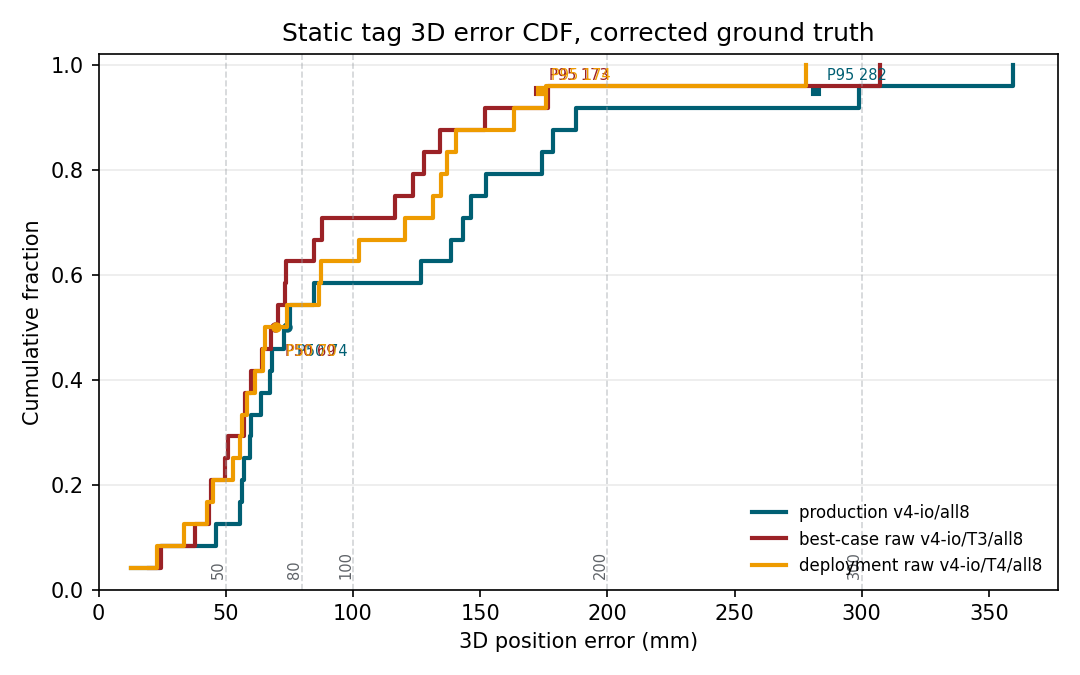
\includegraphics[width=\linewidth]{tag_error_cdf.png}
\caption{Static error CDF from the original FULL analysis.}
\end{subfigure}
\hfill
\begin{subfigure}{0.49\textwidth}
\centering
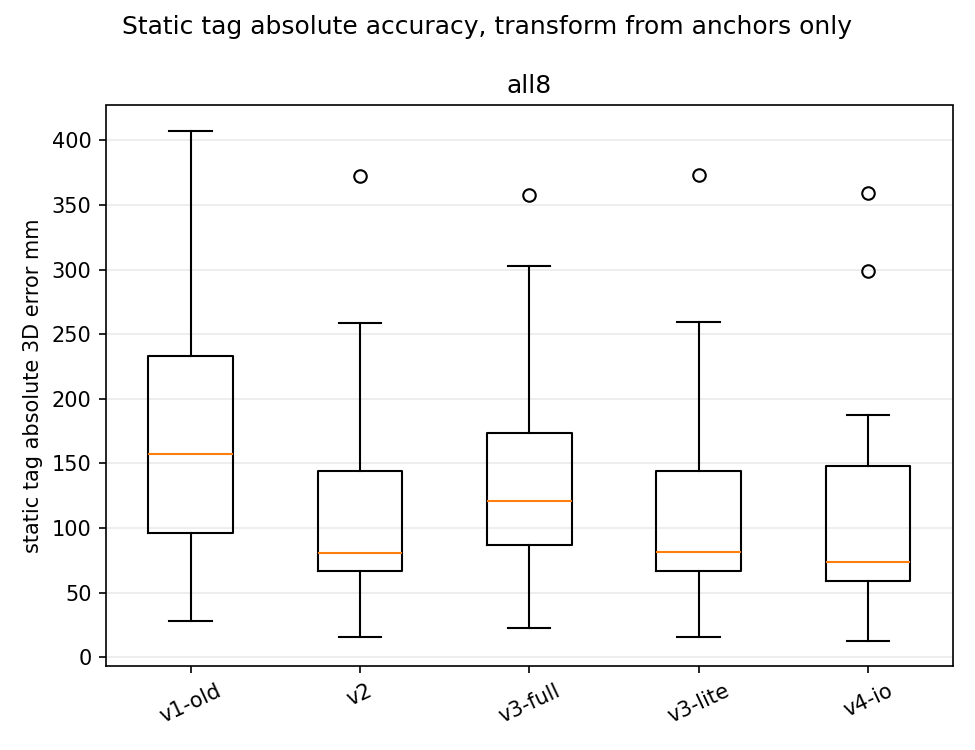
\includegraphics[width=\linewidth]{tag_error_by_position.png}
\caption{Static error by position.}
\end{subfigure}
\caption{Static accuracy has meaningful position dependence and tail behavior;
a single 3D RMSE does not communicate the full structure of the error.}
\end{figure}

\subsection{Static Filtering and Static-Lock Interpretation}

\begin{figure}[H]
\centering
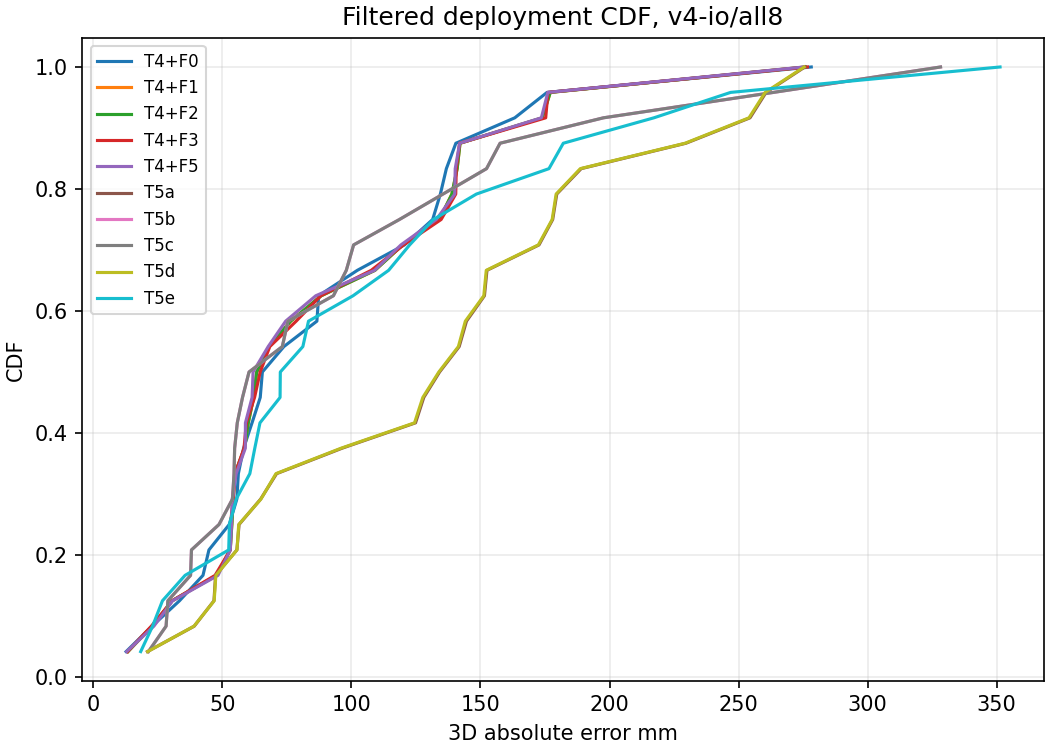
\includegraphics[width=0.8\textwidth]{filtered_static_cdf_v4io_all8.png}
\caption{Static post-solve filtering.  The filter reduces user-facing jitter but
does not eliminate systematic layout/delay/ranging bias.}
\end{figure}

\begin{table}[H]
\centering
\tight
\caption{Static stationary filter results.  These are deployment/static-lock
diagnostics, not raw calibration accuracy.}
\begin{tabular}{lrrrr}
\toprule
Solver & Median & P95 & RMSE & Repeatability SD median \\
\midrule
T4+F0 baseline & 69.7 & 173.9 & 108.9 & 67.4 \\
T4+F5 offline smoother & 64.9 & 175.7 & 109.5 & 18.7 \\
T4+F4 fixed-lag smoother & 65.9 & 176.1 & 109.6 & 21.4 \\
T3+F5 offline smoother & 65.2 & 169.9 & 105.4 & 21.0 \\
\bottomrule
\end{tabular}
\end{table}

Static-lock filtering is valuable if the application knows the tag is stationary:
it reduces the median per-position 3D spread from 67.4 mm to 18.7 mm.  However,
the P95 and RMSE remain close to the unfiltered values because systematic bias
is not removed by smoothing.

\section{Dynamic ROTO Absolute Trajectory Results}

\begin{figure}[H]
\centering
\begin{subfigure}{0.49\textwidth}
\centering
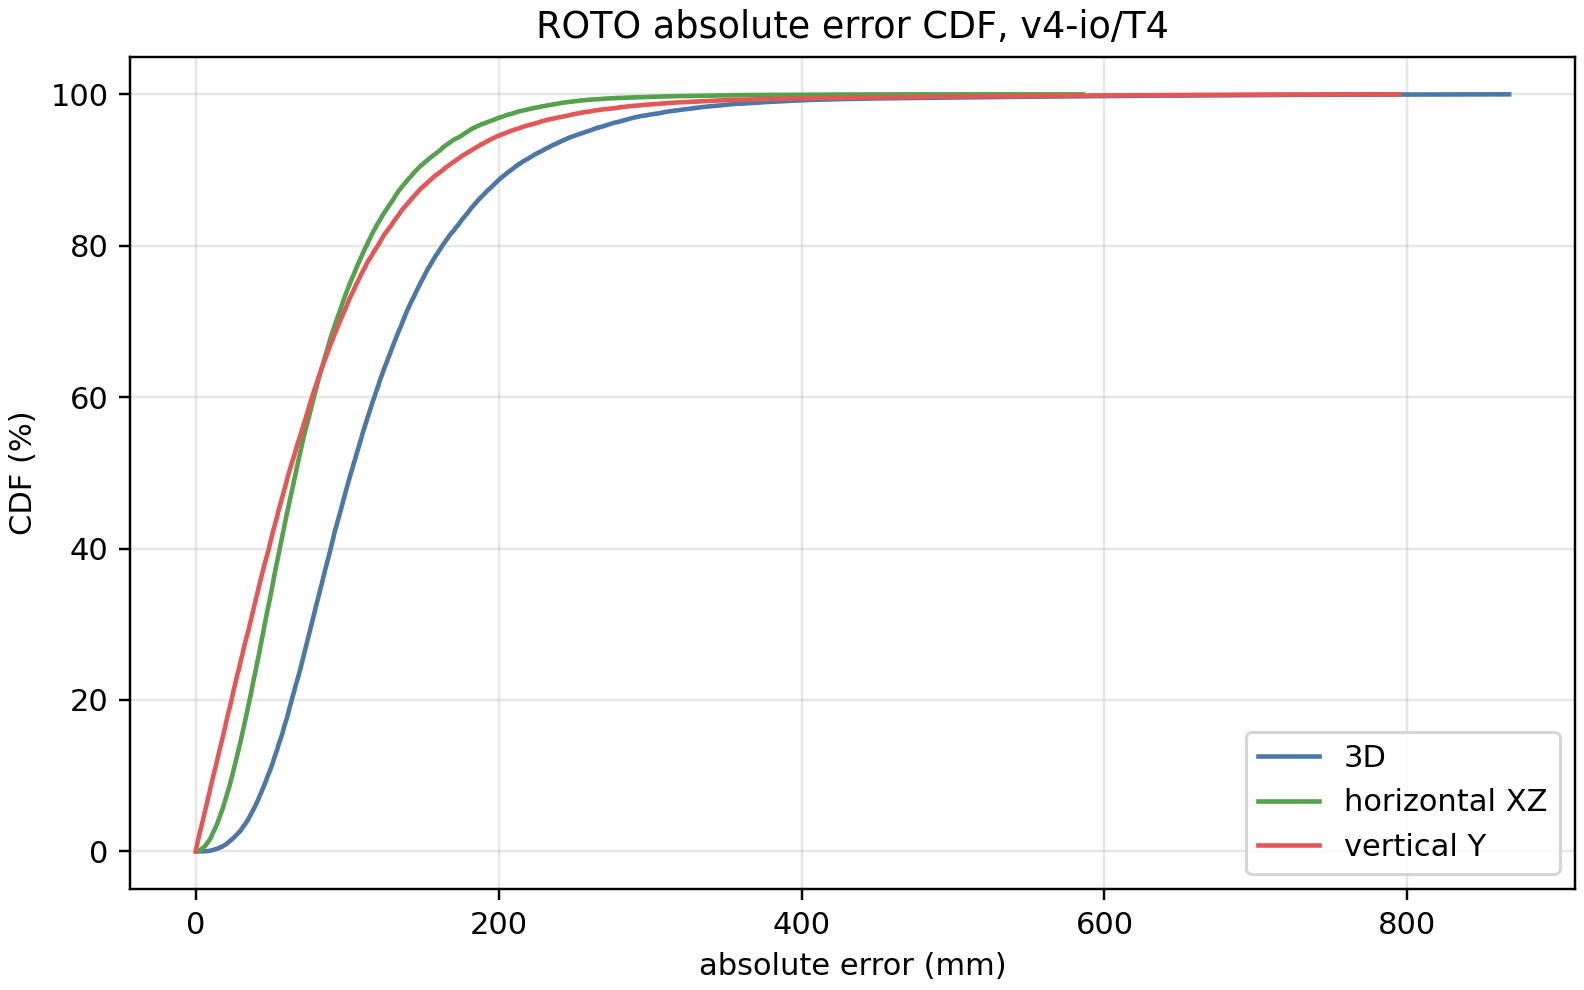
\includegraphics[width=\linewidth]{roto_abs_cdf_v4io_T4.png}
\caption{ROTO absolute error CDF.}
\end{subfigure}
\hfill
\begin{subfigure}{0.49\textwidth}
\centering
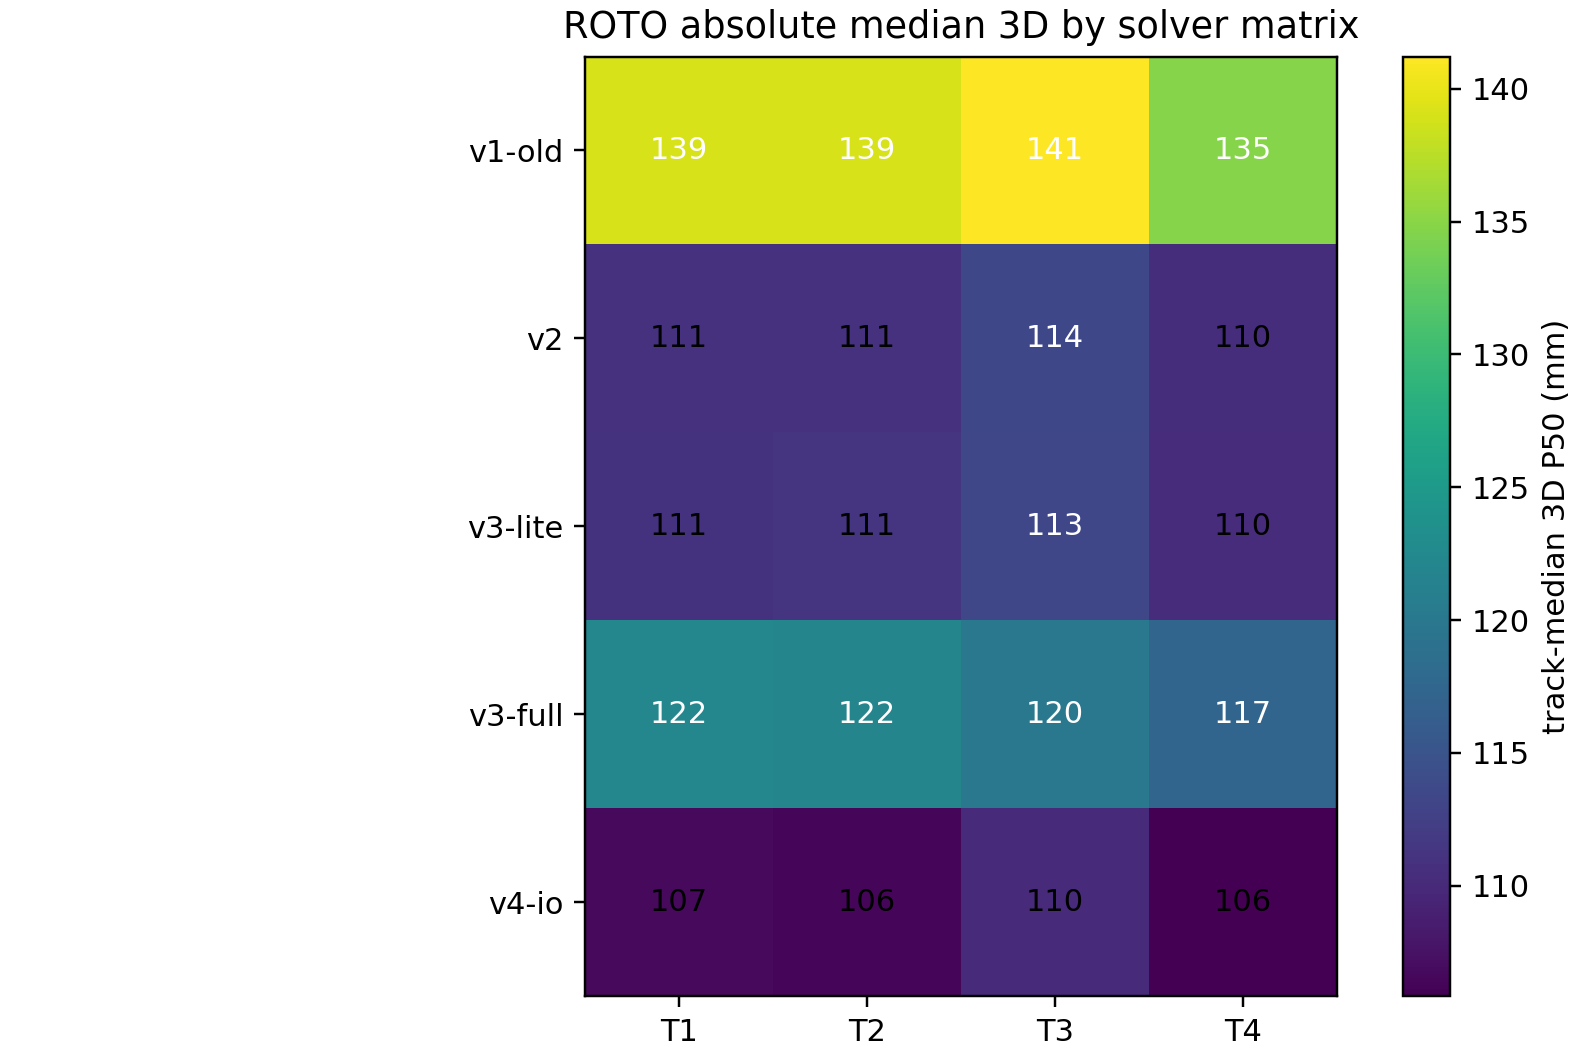
\includegraphics[width=\linewidth]{roto_solver_matrix_median3d.png}
\caption{ROTO solver matrix median 3D error.}
\end{subfigure}
\caption{Dynamic ROTO accuracy remains near 10 cm median even on the same T4 solver
line that performs well statically.}
\end{figure}

\begin{table}[H]
\centering
\tight
\caption{ROTO absolute trajectory accuracy.  P50/P95 are track-median summaries;
RMSE is sample-pooled ATE RMSE.}
\begin{tabularx}{\textwidth}{lXrrr}
\toprule
Case & Layout/delay treatment & Track P50 & Track P95 & Sample RMSE \\
\midrule
FULL original \case{v4-io/T4} & self-cal layout + solver residual corrections & 105.8 & 231.8 & 141.3 \\
Vicon anchors + delaycal & known anchors + re-estimated delay & 105.6 & 200.4 & 125.4 \\
Sim(3) scale + delaycal & global scale removed + re-estimated delay & 110.5 & 200.7 & 127.8 \\
One-baseline E-H + delaycal & one-baseline scale + re-estimated delay & 106.2 & 200.4 & 126.7 \\
Best ROTO median row & one-baseline B-C with solver delay & 100.1 & 220.5 & -- \\
\bottomrule
\end{tabularx}
\end{table}

The key dynamic result is negative but important: the ROTO median does not collapse
when the layout is replaced with Vicon anchors and residual delay is re-estimated.
Static improves from 108.9 mm RMSE to 77.7 mm RMSE under known-anchor delaycal,
but ROTO remains around 105 mm median.  Therefore dynamic ROTO error includes
motion, rotating-wand ranging behavior, antenna/marker geometry, and residual
trajectory effects beyond static infrastructure calibration.

\begin{figure}[H]
\centering
\begin{subfigure}{0.49\textwidth}
\centering
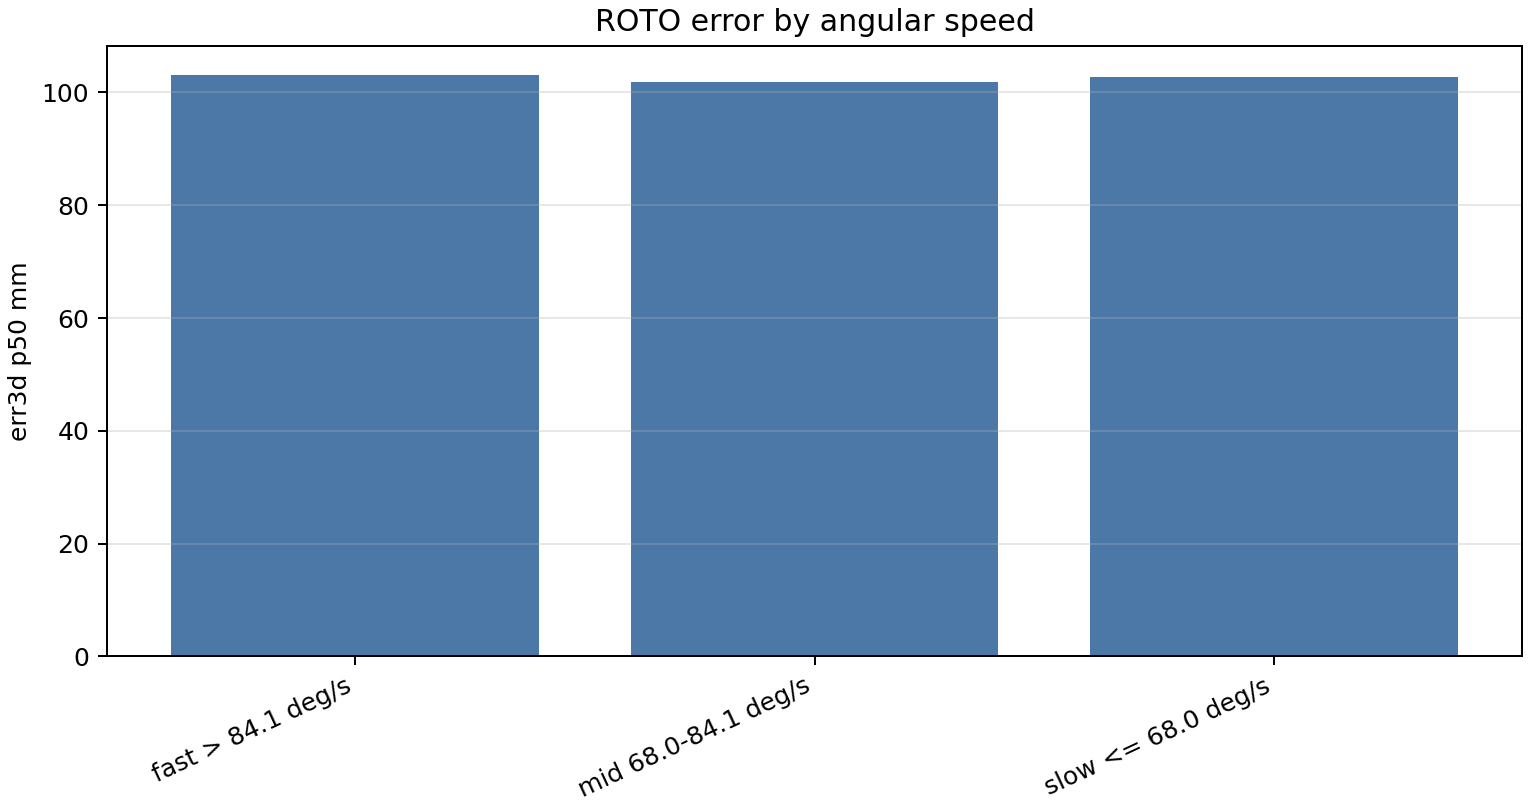
\includegraphics[width=\linewidth]{roto_error_by_angular_speed.png}
\caption{ROTO error by angular speed.}
\end{subfigure}
\hfill
\begin{subfigure}{0.49\textwidth}
\centering
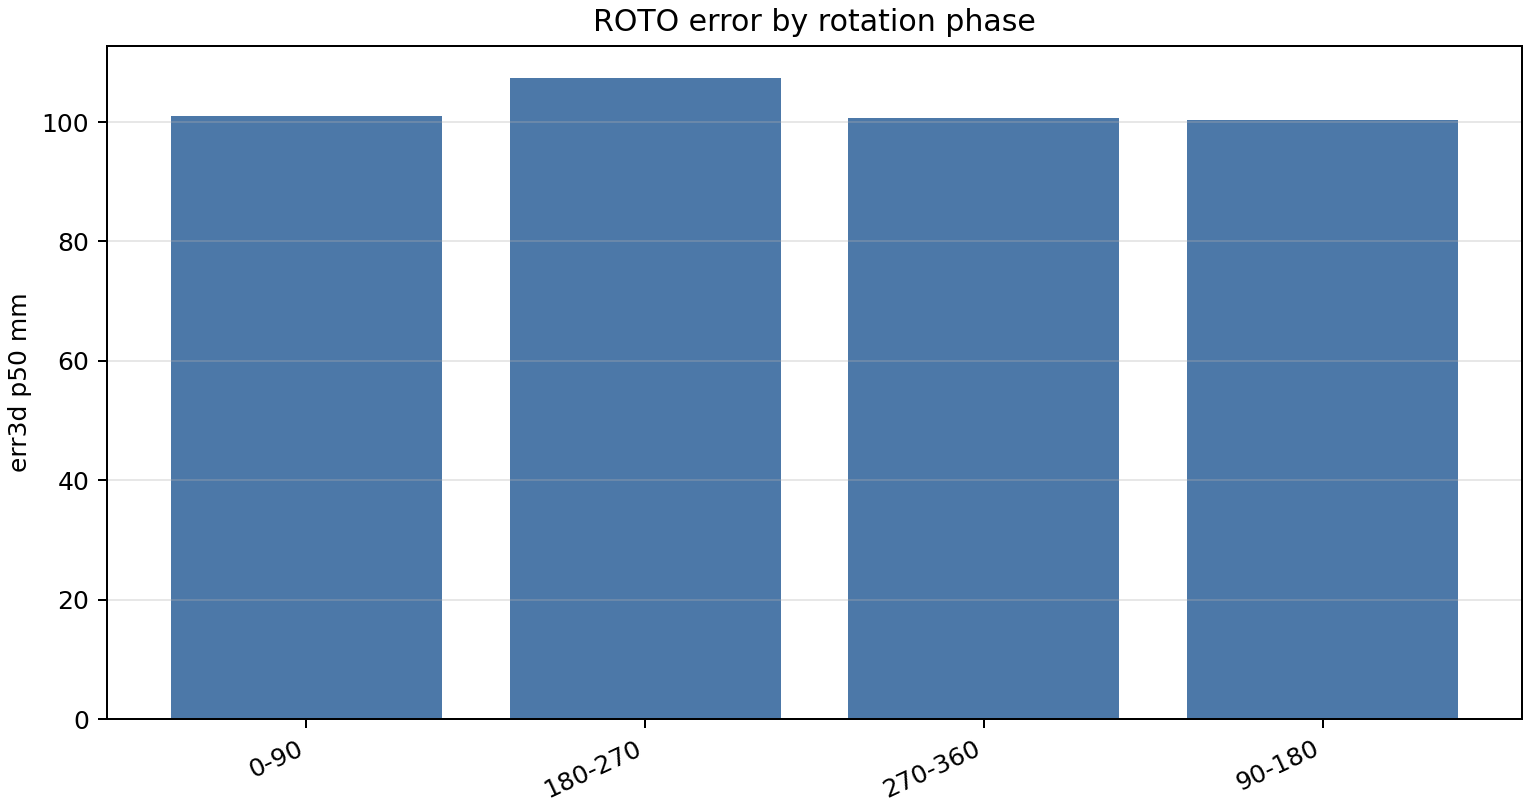
\includegraphics[width=\linewidth]{roto_error_by_phase.png}
\caption{ROTO error by phase.}
\end{subfigure}
\caption{Speed and phase move the median only modestly; they do not explain the
full dynamic residual.}
\end{figure}

\subsection{Time Offset and Clock-Skew Falsification}

The reviewer audit refit one constant time offset per capture, then added an affine
time skew model
\[
t_{\mathrm{query}} = t_{\mathrm{UWB}} + \beta + \alpha (t_{\mathrm{UWB}} - t_{\mathrm{ref}}).
\]
For original FULL \case{v4-io/T4}, the sample-pooled P50 sequence was
102.63 mm at the current beta, 102.69 mm after constant-offset refit, and
102.58 mm after skew refit.  The marginal skew gain was only 0.11 mm pooled P50.
The median fitted skew was -112 ppm with a 228 ppm IQR, and the verdict was
\case{SKEW\_EXCLUDED}.  A 0.8 ms protocol window corresponds to only
0.51 mm median and 0.72 mm P95 displacement at the observed ROTO speeds.

\subsection{Single-Shot Static Versus ROTO}

The static replay was also evaluated at the per-frame level.  For self-cal
\case{v4-io/T4}, static single-shot P50 was 89.6 mm and ROTO single-shot P50 was
102.6 mm, so the dynamic excess in pooled 3D P50 was about 13.1 mm.  Lost static
averaging explains part of the static-vs-dynamic gap, but GDOP-conditioned bins and
component splits still show a limited real dynamic term.  For the Vicon-delaycal
control the dynamic excess is larger, about 24.9 mm P50, again supporting the
conclusion that dynamic ROTO is not only a layout-calibration artifact.

\subsection{Legacy ROTO Self-Consistency and New OptiTrack Center Error}

The old no-groundtruth ROTO self-consistency metrics remain useful but should not
be confused with absolute trajectory error.  Original FULL \case{v4-io/T4} has:
\begin{itemize}
    \item 25.9 mm legacy radius-difference RMS;
    \item 13.7 mm turn-center repeatability median;
    \item 37.6 mm inner/outer center-separation median;
    \item 72.1 mm OptiTrack/Vicon turn-center absolute 3D RMS.
\end{itemize}
The absolute center RMS stays about 72.1 mm for original FULL, 72.7 mm for Vicon
anchors + delaycal, 76.7 mm for full similarity scale + delaycal, and 77.1 mm for
one-baseline E-H + delaycal.

\section{ROTO Filtering and Pseudo-IMU Oracle}

\begin{table}[H]
\centering
\tight
\caption{Post-solve ROTO filtering.  These filters operate on solved positions,
not raw ranges.}
\begin{tabular}{lrrrr}
\toprule
Case & Track P50 & Track P95 & Sample RMSE & Center RMS \\
\midrule
FULL F0 baseline & 105.8 & 231.8 & 141.3 & 72.1 \\
FULL F4 fixed lag & 86.3 & 158.2 & 103.1 & 69.1 \\
FULL F5 offline RTS & 83.3 & 148.6 & 98.9 & 68.3 \\
Vicon F0 baseline & 105.6 & 200.4 & 125.4 & 72.7 \\
Vicon F4 fixed lag & 84.0 & 145.4 & 95.1 & 70.5 \\
Vicon F5 offline RTS & 82.7 & 139.1 & 91.2 & 70.0 \\
\bottomrule
\end{tabular}
\end{table}

Fixed-lag and offline smoothing reduce dynamic scatter substantially, but this is
a trajectory-output/latency tradeoff.  The calibration-level claim should keep the
unfiltered ROTO result, while F4/F5 should be reported as deployment-filter or
offline upper-bound diagnostics.

\begin{table}[H]
\centering
\tight
\caption{Pseudo-IMU oracle replay.  The motion prior is derived from OptiTrack
marker motion and is lever-armed to the UWB antenna point.}
\begin{tabular}{lrrrrr}
\toprule
Case & Fusion & Track P50 & Track P95 & Sample RMSE & dR RMS \\
\midrule
FULL original & PI0 baseline & 105.8 & 231.8 & 141.3 & 25.9 \\
FULL original & PI1 causal oracle & 66.1 & 97.5 & 71.6 & 12.3 \\
FULL original & PI4 offline oracle & 58.7 & 81.5 & 61.8 & 5.3 \\
Vicon delaycal & PI0 baseline & 105.6 & 200.4 & 125.4 & 18.0 \\
Vicon delaycal & PI1 causal oracle & 64.0 & 100.2 & 69.8 & 11.7 \\
Vicon delaycal & PI4 offline oracle & 59.9 & 82.0 & 63.1 & 4.3 \\
\bottomrule
\end{tabular}
\end{table}

The body-fit antenna prior residual is only 0.6 mm P50-of-P50 and 1.5 mm
P50-of-P95 across tracks, so the pseudo-IMU is not accidentally using the marker
body centroid as the antenna point.  It is still an oracle: it uses OptiTrack-derived
motion, not a real IMU.  The correct paper framing is that a properly lever-armed
real inertial relative-motion channel is worth implementing and validating in a
raw-range EKF/UKF, not that the current system already has a deployable UWB+IMU
result.

\section{Robustness and Reporting Checklist}

\begin{table}[H]
\centering
\tight
\caption{Numerical precision and dropout stress.  Bootstrap values are not independent
deployment repeatability.}
\begin{tabularx}{\textwidth}{lXrrrr}
\toprule
Case & Diagnostic & Coord SD & Delay rel-A SD & Static P50/P95 & Note \\
\midrule
Original self-cal & raw-pair median bootstrap & 1.02 & 0.56 & 76.3/180.9 & within-campaign sampling SE \\
Vicon truth + delaycal & residual-delay bootstrap & 0.00 & 0.45 & 65.0/126.7 & coordinate fixed by control \\
Sim(3) scale + delaycal & raw-pair median bootstrap & 0.97 & 0.53 & 69.3/134.8 & within-campaign sampling SE \\
One-baseline E-H & raw-pair median bootstrap & 1.20 & 0.54 & 60.6/127.9 & within-campaign sampling SE \\
\bottomrule
\end{tabularx}
\end{table}

The raw-pair bootstrap result is intentionally not called deployment repeatability.
It agrees with the analytical median sampling standard error and therefore measures
large-\(n\) numerical precision inside the same campaign.  Independent repeated
AutoPos deployments, repeated-run delay standard deviations, PANS/manual baselines,
explicit CIR/NLOS labels, and raw dynamic packet-loss re-solves remain separate
evidence gaps.

Synthetic static dropout was re-solved from raw static frames.  Random per-frame
four-anchor stress degrades original self-cal from 76.3/180.9 mm to 87.7/292.4 mm
position P50/P95, with much worse sample-level spread.  Fixed random four-anchor
subsets and best-GDOP four-anchor subsets make non-convergence explicit; their P50/P95
values are conditional on convergence.  ROTO packet stress is solved-sample thinning,
not a raw range re-solve: ATE remains stable under thinning, while RPE worsens as
effective update rate drops from about 10 Hz to about 1 Hz.

\section{Per-Tag and Per-Anchor Residual Structure}

The WHY \#9 two-way median-polish decomposition separates common-mode, tag main
effects, anchor main effects, and tag-anchor interactions.  Pairwise tag residual
range offsets are stable across self-cal and Vicon-delaycal scenarios:
\begin{itemize}
    \item BS2DCE minus BSF66F: 31.0 mm in self-cal, 34.6 mm in Vicon-delaycal;
    \item BSDC91 minus BSF66F: -12.7 mm in self-cal, -11.7 mm in Vicon-delaycal;
    \item BS2DCE minus BSDC91: 43.7 mm in self-cal, 46.3 mm in Vicon-delaycal.
\end{itemize}
The maximum cross-scenario change of these tag differences is only 3.6 mm, and
the median interaction terms are 0.9 mm and 2.4 mm.  These are clean deployable
per-tag range-offset trim targets.  They should not be over-named as antenna delay;
they combine device antenna delay, fixed installation effects, and stable power or
range-bias terms into one scalar correction.

The anchor side is different.  Absolute per-anchor and per-tag delay are not
identifiable from tag-to-anchor ranges alone because of global delay/scale gauge
coupling.  The self-cal anchor residual structure absorbs layout radial error
almost one-to-one, so self-cal \case{d\_anchor} should be reported as a layout-level
residual correction, not a physical anchor antenna-delay measurement.

\section{Recommended Claims}

\begin{enumerate}
    \item Use the unfiltered production mean-aggregated \case{v4-io/T4} result as
    the deployed static headline: \textbf{72.7 mm median, 171.5 mm P95, 109.8 mm RMSE}.
    \item Report \case{69.7/173.9 mm} only as a median-estimator ablation on the same
    solver line, not as the deployed production output.
    \item Report FULL-US as the BioSpur UWB+US30 deployment-gauge variant.  It should
    not be claimed as a major accuracy improvement over FULL under legacy
    anchor-locked metrics; its contribution is fixing the physically interpretable
    vertical gauge.  Quote the height-preserving \case{v4-io} static diagnostic as
    \textbf{72.5/284.8 mm}, RMSE \textbf{139.1 mm}.
    \item State the known-anchor + re-estimated-delay control as a diagnostic control,
    not as a plain lower bound: it is the best static control at 64.1/128.4 mm and
    77.7 mm RMSE, but it requires OptiTrack anchors and re-estimated residual delay.
    \item Present delay-layout coupling as a core result: the 311/252/77 mm triangle
    and the \(R^2=0.998\), slope \(-0.982\) radial-absorption mechanism are two views
    of the same non-separability.
    \item State ROTO conservatively: unfiltered dynamic absolute trajectory error is
    about 10 cm median, with P95 about 20--23 cm depending on the control row.
    \item Treat F4/F5 filtering and PI1/PI4 pseudo-IMU results as deployment-filter
    diagnostics or oracle upper bounds, not calibration accuracy.
    \item Do not report only one 3D RMSE.  Split repeatability, absolute error, scale
    bias, shape distortion, delay-layout coupling, downstream tag error, and tail behavior.
\end{enumerate}

\section{Limitations and Next Experiments}

The present dataset covers the corrected OptiTrack-isolated FULL analysis in depth,
but it still lacks several independent evidence streams:
\begin{itemize}
    \item independent repeated AutoPos deployments or layout splits;
    \item true repeated-run residual-delay standard deviation;
    \item a practical PANS/manual baseline in the same dataset;
    \item explicit CIR/NLOS labels tied to each link;
    \item raw dynamic ROTO range re-solve under physical packet loss;
    \item real IMU data with calibrated IMU-to-UWB-antenna extrinsics.
\end{itemize}

The most valuable next experiment is a real UWB+IMU fusion run.  The pseudo-IMU
oracle shows that a correctly lever-armed relative-motion prior has enough leverage
to bring ROTO from 105.8/231.8 mm to 66.1/97.5 mm in the strong causal oracle case.
The deployable version should use real inertial measurements, an antenna-frame
extrinsic calibration, and a raw-range EKF/UKF rather than only smoothing solved
positions.

\section{Source Artifacts}

This LaTeX report is based on the following generated artifacts:
\begin{itemize}
    \item \case{FULL\_4way\_comparison/reports/FULL\_4WAY\_BIG\_COMPARISON.md}
    \item \case{FULL\_4way\_comparison/reviewer\_audit/reports/MEASUREMENT\_REVIEWER\_AUDIT.md}
    \item \case{FULL\_4way\_comparison/reporting\_checklist/reports/REPORTING\_CHECKLIST\_AUDIT.md}
    \item \case{FULL\_4way\_comparison/resilience\_gap\_audit/reports/RESILIENCE\_GAP\_AUDIT.md}
    \item \case{FULL\_4way\_comparison\_US/reports/FULL\_4WAY\_BIG\_COMPARISON.md}
    \item \case{FULL\_NO\_US\_VS\_US/reports/FULL\_NO\_US\_VS\_US\_COMPARISON.md}
    \item \case{FULL\_4way\_comparison/tables/full\_4way\_headline\_comparison.csv}
    \item \case{FULL\_4way\_comparison/reporting\_checklist/tables/*.csv}
    \item \case{FULL\_4way\_comparison/reviewer\_audit/tables/why*.csv}
\end{itemize}

\end{document}
